\def\QRCODE{TB_image_TUT.IMG.image_characterization_matlabqrcode.png}
\def\QRPAGE{http://www.iptutorials.science/tree/master/TB_image/TUT.IMG.image_characterization/matlab}
\mcorrectionsection{Matlab correction}

\subsection{Perimeters}
The convolution is used here as an easy way of getting the borders of the object in one direction, i.e. counting the number of intercepts. This method is efficient because, for one given direction, a high number of lines are considered.

\begin{matlab}
% load the image
I = imread('camel-5.png');
I=double(I)>0; % ensure binarization
imshow(I)

% defines an orientation, computes the number of intercepts by convolution
h = [-1 1];
b = abs(conv2(double(I), h, 'same'));
n1 = sum(b(:))/2;

b = abs(conv2(double(I), h', 'same'));
n2 = sum(b(:))/2;

% diagonal orientations:
h = [1 0; 0 -1];
b = abs(conv2(double(I), h, 'same'));
n3 = sum(b(:))/2;
h = [0 1; -1 0];
b = abs(conv2(double(I), h, 'same'));
n4 = sum(b(:))/2;

% crofton evaluation and comparison
perim_Crofton = pi/4 * sum( [n1 n2 n3/sqrt(2) n4/sqrt(2)])

perim_usual = sum(sum(bwperim(I)))
\end{matlab}

The \minline{b} matrix obtained for intercept evaluation is illustrated in Fig.\ref{fig:image_characterization:matlab:edges}. The results obtained are:
\begin{mwindow}
perim_Crofton =
   1.3055e+03

perim_usual =
        1182
\end{mwindow}

\begin{figure}[htbp]
\centering
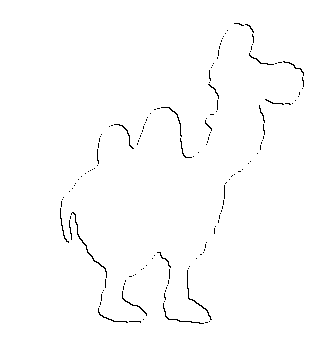
\includegraphics[width=5cm]{contours_diag_1.png}
\caption{Illustration of the intercept number evaluation in the first diagonal direction.}
 \label{fig:image_characterization:matlab:edges}
\end{figure}


\subsection{Feret diameter}
The code consists in rotating the image and evaluating the projected diameter. The rotation function can interpolate the pixel, a binarization step is thus required. The function \minline{sum} indirectly performs the projection as it sum all values in one direction only.

\begin{matlab}
% discrete orientations
deg = 1:180;
for i = 1:length(deg)
   I2 = imrotate(I,deg(i),'nearest');
   I3 = sum(I2)>0;
   diameter(i) = sum(I3); 
end

diamFeret_min = min(diameter)
diamFeret_max = max(diameter)
diamFeret_mean = mean(diameter)
\end{matlab}

For the camel image, the Feret diameters are:
\begin{mwindow}
diamFeret_min =
   184

diamFeret_max =
   326

diamFeret_mean =
  267.1944
\end{mwindow}

\subsection{Circularity}
For a disk, the perimeter is $\pi\cdot D$ and the surface is $\pi\cdot\frac{D^2}{4}$.

In order to generate a binary image containing a disk, one simple way is to use the formula:
$(x-x_0)^2+(y-y_0)^2\leq R^2$.
This gives with matlab, for an image of size $1000\times 1000$, a circle of radius 400 centered in $(500,500)$:
\begin{matlab}
I = zeros(1000,1000);
[X,Y] = meshgrid(1:1000,1:1000);
I = sqrt((X-500).^2+(Y-500).^2) < 400;
\end{matlab}
The perimeters are evaluated with the code proposed earlier.  The results are show that the Crofton perimeter is more precise in this example.
\begin{mwindow}
>> 2*pi*400
ans =
   2.5133e+03

>> perim_Crofton =
   2.5113e+03

>> perim_usual =
   2260
   
>> circ_Crofton =
    1.0015

>> circ_usual =
    1.2366
\end{mwindow}

\subsection{Convexity}
In order to compute the convexity criterion, the convex hull is computed. For this purpose, all the pixels of the objects are converted into points. The polygon is then transformed into a binary image. The resulting image of the convex hull is presented in Fig.\ref{fig:image_characterization:matlab:convhull}.
\begin{matlab}
I = imread('camel-5.png');
I = double(I)>0;

dim = size(I);
D1  = dim(1);
D2  = dim(2);

[Y,X] = find(I==1);
CH = convhull(X,Y);
XCH = X(CH);
YCH = Y(CH);
I_convhull = poly2mask(XCH,YCH,D1,D2);

figure
subplot(121);imshow(I);
subplot(122);imshow(I_convhull)

convexity = sum(I(:))/sum(I_convhull(:))
\end{matlab}
\begin{mwindow}
convexity = 0.6439
\end{mwindow}

\begin{figure}[htbp]
\centering
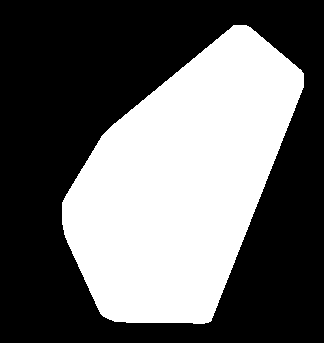
\includegraphics[width=5cm]{convhull_camel.png}
 \caption{Convex hull of the camel object.}
 \label{fig:image_characterization:matlab:convhull}
\end{figure}
